\section{Contrucci�n de interfaces de usuario usando el patr�n MVC}

\subsection{MVC}

Modelo Vista Controlador (MVC) es un patr�n de arquitectura de software que
separa los datos de una aplicaci�n, la interfaz de usuario, y la l�gica de
negocio en tres componentes distintos.

El estilo fue descrito por primera vez en 1979 por \emph{Trygve Reenskaug},
entonces trabajando en Smalltalk en laboratorios de investigaci�n de Xerox. 
La implementaci�n original est� escrita en Programaci�n de Aplicaciones en 
Smalltalk-80(TM): Como utilizar Modelo Vista Controlador.

La idea principal de MVC, y que influy� a frameworks de presentaci�n posteriores,
es la de Presentaci�n Separada \emph{(Separated Presentation)} que consiste en
hacer unadivisi�n clara entre objetos de dominio que modelan nuestra percepci�n 
del mundo real y objetos de presentaci�n que son los elementos Interfaz de
usuarios que vemos en lapantalla.\\

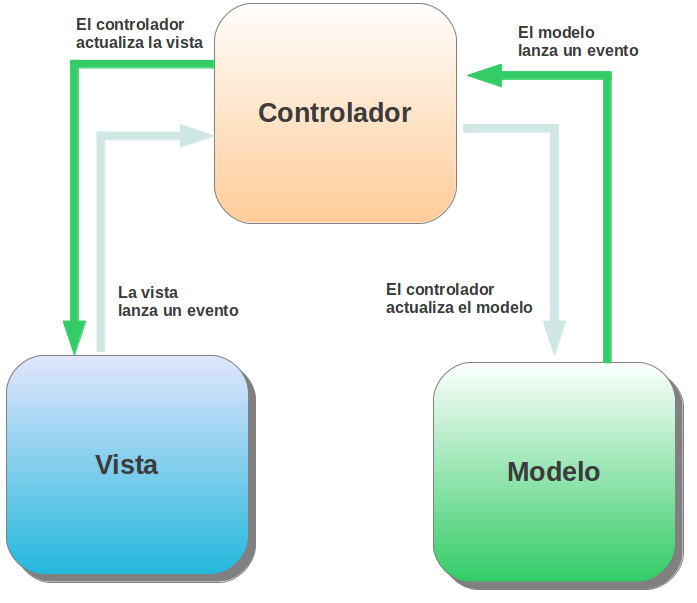
\includegraphics[width=300px, height=300px]{img/mvc}

\begin {itemize}


  	

\item {\bf Modelo}
	El modelo maneja el comportamiento y los datos del dominio de la aplicaci�n,
	responde a los pedidos de informacion sobre su estado (por lo general de la
	vista), y responde a las instrucciones para cambiar su estado (por lo general
	desde el controlador). Tambi�n deber�an ser capaces de soportar	m�ltiples presentaciones
	
	
\item {\bf Vista}
	Muestra la informacion del modelo al usuario. 
	
\item {\bf Controlador}
	Es el intermediario entre el modelo y la vista.
	Mapea acciones del usuario con acciones al modelo.
		
	
\end {itemize}

\subsection{Eventos}

TODO\\

\subsection{Binding}
El Binding permite sincronizar los valores de las propiedades de dos objetos
diferentes (vista y modelo). Cada vez que el valor de una propiedad
cambia, el objeto notifica (lanza un evento), y todas las
propiedades que esten bindeadas a el reflejan los cambios automaticamente\\


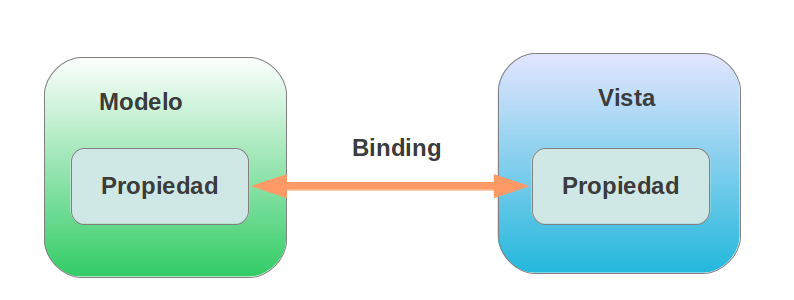
\includegraphics[width=300px]{img/binding}

Asociando estas dos propiedades, el flujo entre ambos puede asociarce en dos
modos.

\begin {itemize}

\item {\bf OneWay}
Con este tipo de binding el flujo de datos se realiza en una sola direcci�n. 

\item {\bf TwoWay}
En este tipo de asociaci�n el flujo se produce en ambas direcciones. Los cambios
realizados en el modelo se ven reflejados  en la vista y viceversa. (Este es el
tipo de binding que tenemos en el Arena)

\end {itemize}

\subsubsection{Ventajas}
Al tener vinvulados los datos entre la interfaz y el modelo

\subsubsection{DesVentajas}
Al no existir esa vinculacion, los datos que se tienen que pasar del modelo a la
interfaz y viceversa , hay que hacerlo a mano.


\subsubsection{Problemas sin binding}
Al no tener binding perdemos mucho tiempo de desarrollo en  traspasar los datos
de los objetos de dominio hacia los componentes de la interfaz grafica y
viceversa.

\subsubsection{Problemas con Binding}
Un problema que aparece frecuentemente es que el binding en su versi�n m�s 
sencilla modifica los objetos directamente, por lo que al cancelar una operaci�n 
se debe volver al estado anterior, y este proceso es repetitivo y propenso a errores. 
Con frecuencia implica introducir comportamiento propio de la interfaz de
usuario, en mis objetos de dominio, mezclando la l�gica de las dos partes de
la aplicaci�n. Esto me obliga a adaptar mi dominio a este sistema, y repetir
muchas l�neas de c�digo.
	
\section{Transacciones}	
{TODO} como enganchar lo anterior con esto\\

Las transacciones en un entorno de bases de datos tienen dos propositos
principales:

\begin {itemize}

  \item	
  Proveer unidades de trabajo confiables, que permitan mantener la consistencia
  incluso si el sistema falla.
  
  \item
  Proporcionar un aislamiento entre los programas de acceso a una base de datos
  al mismo tiempo.
  
\end{itemize}

�Que pasa con las aplicaciones orientadas a objetos?
\begin {itemize}

  \item
  	Las unidades de trabajo y el aislamiento siguen siendo utiles en programacion
  	orientada a objetos.
  	
  \item
  	Pero la separacion entre el programa y la base de datos es contraria a los
  	principios de la programacion orientada a objetos.
\end{itemize}	

El objetivo de este trabajo es proponer una soluci�n a estos dos problemas que
minimice el impacto en el c�digo de las clases del dominio de la aplicaci�n


